\chapter{Implementation}
    \label{chap:implementation}

   This chapter will explain my implementation for this project. It will first give an overview of the architecture of the software product. After that, we will present each one of the challenges that have been implemented so far.

    \section{Architecture} 
        \label{sec:architecture}
        
    The central part of the software implementation consists of the Damn Vulnerable Mobile - Inter Component Communication app. This Android app contains all of the educational material needed to understand Android ICC and complete each challenge, encourages the user to learn interactively,  and it provides access to each challenge and to settings to control the challenge or the learning experience. 
    
    The rest of the project consists of a series of Android apps that play the role of either a vulnerable app or a malware. These apps are made to appear to be authentic apps with real-world functionalities, though many of them are nowhere close to full-feature app. Each challenge consists of an authentic scenario of a malware app attacking one of the vulnerable apps through one particular ICC vulnerability.
    
    The DVM-ICC app communicates with the challenge apps through the use of files in order to apply various settings to control the behaviour of the apps. These settings are explained in subsection \ref{subsec:challenge_settings}. Moreover, each pair of vulnerable and malicious apps communicate between each other as a result of the cyber attack, through the medium of Intents. The manner in which this communication takes place will be explained in detail for each challenge in section \ref{sec:challenges}.
    
    \section{DVM-ICC Application}
        \label{sec:home_app}
        
    In this section, I will explore the features of the DVM-ICC Android app. While doing so, I will explain the intended workflow that a user needs to follow and how app provides an educational experience. The follow description applies to the Beginner mode. The app has three different operation modes, which will be fully explained in subsection \ref{subsec:challenge_modes}.
    
    \subsection{Home Menu}
        \label{subsec:home_menu}
        
    \begin{wrapfigure}[15]{r}{0.3\textwidth}
        \centering
        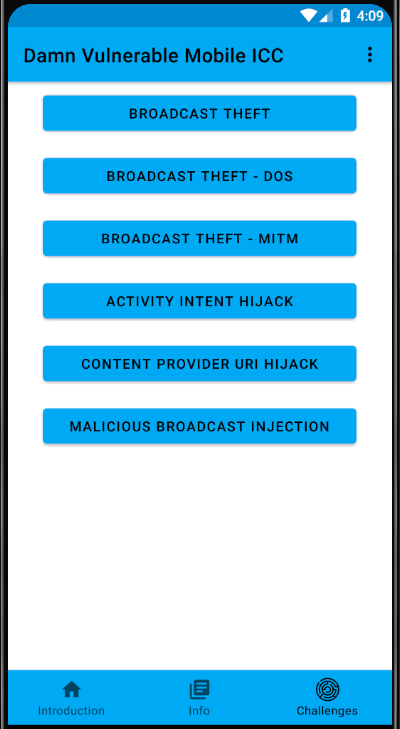
\includegraphics[width=0.3\textwidth]{graphics/home_activity.PNG}
        \caption{The first menu in the DVM-ICC app.}
        \label{fig:home_menu}
    \end{wrapfigure}
        
    The first screen the user sees when starting the app has 3 sub-pages: Introduction, Info and Challenges, as you can see in figure \ref{fig:home_menu}. The Introduction page gives an introduction of the project and explains the intended workflow for using the product. The Info page provides all of the necessary technical background to understand ICC vulnerabilities and attacks. It covers what components and permissions are, how components communicate between each other and the major types of ICC based attacks: Intent Hijacking and Intent Spoofing. The Challenges page lets the user select what challenge they want to start, as shown in figure \ref{fig:home_menu}.
    
    \subsection{Challenge Settings}
        \label{subsec:challenge_settings}
        
    When clicking on a challenge, the user is taken to a menu where they can change the settings that define how the challenge will be undertaken. Here, you can set the operation mode for the challenge. Moreover, the user can enable or disable the malware of the selected challenge. If disabled, the malicious app will not perform any cyber-attack and therefore it will not interfere with any vulnerable app or the rest of the system.
    
    The most important setting on this screen is the security level of the vulnerable app. Inspired from DVWA, as described in subsection \ref{subsec:ICC_related_work}, these levels define how secure the vulnerable app is against attacks from the malware. Each challenge's vulnerable app has between 2 and 5 security levels, with each successive level using more secure code. This culminates with the Impossible level, where the vulnerability is fixed and the malware can not perform the attack. When the malware is enabled, it will overcome the defences of the current security level, except for the Impossible level. The number of security levels and their meaning depends on the challenge. In general, each security level means that a component or broadcast is protected with a more powerful permission, that components are no longer exported or that an intent is now sent explicitly. 
    
    These settings are written to a text file that is located in the DVM-ICC's app specific directory on the device's external storage, from where it can be accessed by any other app, including the other apps that are part of this project. The security level setting will dynamically change the behaviour of the vulnerable and malicious apps, and the user does not need to restart them, with some
    exceptions. The challenge settings can be changed at any time while doing a challenge.
    
    \subsection{Identifying the malware and the vulnerable app}
        \label{subsec:identify_challenge_apps}
        
    \begin{wrapfigure}[19]{r}{0.4\textwidth}
        \centering
        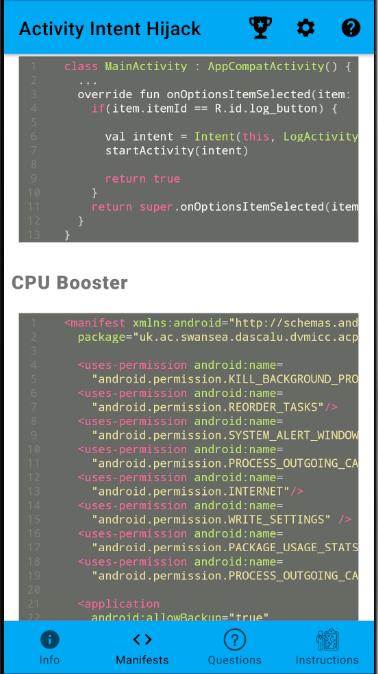
\includegraphics[width=0.4\textwidth]{graphics/manifests.PNG}
        \caption{The Manifests page in the Challenge activity.}
        \label{fig:manifests_fragment}
    \end{wrapfigure}
        
    Once the user applies the settings described in subsection \ref{subsec:challenge_settings}, the application starts the Challenge activity, which you can see in figure \ref{fig:manifests_fragment}. The first task of every challenge is to identify the pair of vulnerable and malicious apps for that challenge from amongst all of the apps that are part of the project, except the DVM-ICC app itself. 
    
    The Info page gives a technical description of one of the two major attack categories, Intent Hijacking or Intent Spoofing, followed by a detailed description of the specific cyber attack related to this challenge. After reading and understanding this information, the user needs to go the Manifests page, where they can view for each app the contents of its manifest and all snippets of code that sends intents, as shown in figure \ref{fig:manifests_fragment}. Based on the technical background the user was given in the Info page and in the Home Menu from subsection \ref{subsec:home_menu}, they need to look through the code in the Manifests page and try to identify the vulnerable app and the malware for this challenge. 
    
    The user should be able to detect vulnerable apps by looking for intents being sent implicitly or for exported components, for example. Malwares can be usually identified by the use of intent filters matching intents that are only sent by a vulnerable app, or by sending an explicit intent to another app that is part of this project. The features that identify the vulnerable app and the malware depend on the selected challenge.
    
    The Questions page contains text boxes where the user can type in their answers and be told if they have correctly identified the apps.
    
    \subsection{Performing the cyber-attack}
        \label{subsec:perform_attack}
        
    Now that the user knows the correct pair of apps for this challenge, the next task of the challenge is to use these apps to witness the cyber-attack take place.
    
    \begin{wrapfigure}[20]{r}{0.4\textwidth}
        \centering
        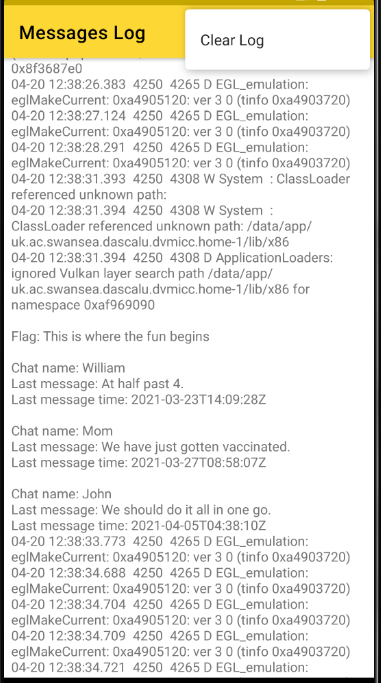
\includegraphics[width=0.4\textwidth]{graphics/log.PNG}
        \caption{Log of the malware for Content Provider URI Hijack after it successfully attacked the vulnerable app.}
        \label{fig:malware_log}
    \end{wrapfigure}
    
    Once you have correctly answered the questions regarding the identity of the malware and vulnerable app, the Instructions page will display detailed instructions for using the apps such that the specific cyber-attack for that challenge will take place. This page can be accessed from the activity shown in figure \ref{fig:manifests_fragment}.
    
    In general, the user is asked to take a look at the two apps to familiarise themselves with them and what they can do. Then, the user should make sure that the security level is set to low. After that, they should use the vulnerable app and malware according to the provided instructions in order to trigger the attack and observe it. 
    
    Following that, the user needs to go the malware and look in its Log, which is accessed from its app bar. If the attack was successful, the malware should have written in its log the flag associated with this specific challenge and security level, along with any relevant data it managed to steal from the vulnerable app. These would be hidden amongst the output of Android Log. 
    
    You can see an example of this in figure \ref{fig:malware_log}, where the messages from the Whatsapp vulnerable app have been stolen by the SMS Messages malware. The user should then copy the flag and submit it to the flag question for the current security level in the Questions page in the DVM-ICC app, to prove they have completed one level of the challenge. 
    
    At this point, the user should clear the log of the malware, to see the effects of the next attack more easily, and then change the security level to the next value. They should repeat the process described in this subsection for every security level of that challenge.
    
    Through performing the task described in this section, the user will witness an example of a cyber attack happening in an authentic scenario, with a real malicious app exploiting an insecure app. 
    
    \subsection{Security Levels Explanation}
        \label{subsec:security_levels_explanation}
        
    \begin{wrapfigure}[22]{r}{0.45\textwidth}
        \centering
        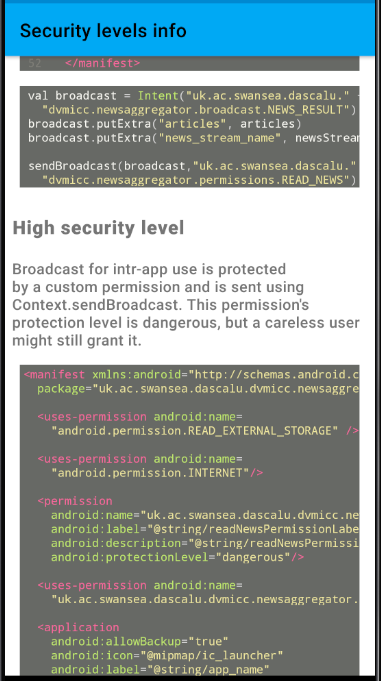
\includegraphics[width=0.45\textwidth]{graphics/security_level_explanation.PNG}
        \caption{Part of the explanation of the security levels for the Broadcast Theft Challenge.}
        \label{fig:security_levels}
    \end{wrapfigure}
        
    While completing the task described in subsection \ref{subsec:perform_attack}, the user can click on the Help button that you can see at the top right in figure \ref{fig:manifests_fragment} to view an explanation of the security levels for the current challenge. This view is hidden until the user has identified the pair of apps for the current challenge, as explained in subsection \ref{subsec:identify_challenge_apps}.
    
    For each level, it will explain how it works and how it is more secure than the previous level. Following this explanation is a view of the full manifest of the vulnerable app, as it would be used for that security level. Finally, this view might show code snippets that introduce a vulnerability through the way they send an intent.
        
    You can see part of the Security Levels explanation for the Broadcast Theft challenge in figure \ref{fig:security_levels}, as an example. The top code snippet shows the code used to send a broadcast in the News Aggregator app in the medium security level. Since this code send the broadcast implicitly, it is insecure.
    
    This activity teaches the user how and where the vulnerability is introduced and what steps a programmer can take to secure the vulnerable app, complete with code examples from the app itself. Some solutions fail to completely remove the vulnerability, and this activity teaches the developer why they are inadequate. The explanation of the Impossible level shows how to completely remove the attack surface.
    
    By looking at these explanations while performing the task described in subsection \ref{subsec:perform_attack}, the user will be able to see how the cyber attack of that challenge can still succeed despite the programmer implementing some security defences.
    
    \subsection{Challenge Conclusion}
        \label{subsec:challenge_conclusion}
    
    Once the user has performed the cyber attack and has submitted the correct flag for every security level, they have completed that challenge. As a reward, they can now click on the trophy button on the app bar of the Challenge activity, which you can see in figure \ref{fig:manifests_fragment}.
    
    This will open an activity where the user can read the conclusion to the current challenge. This text will give a summary of the whole challenge, going through how the vulnerability is introduced, how the attacker can create a malware that takes advantage of it, and how to fix the vulnerability. Moreover, the conclusion will comment on the authenticity of the scenario presented in the challenge, covering how or why the vulnerability was introduced in the first place and how likely it is for the scenario might to be encountered in the real world. The purpose of this conclusion is condense all of the information that the user should take away from this challenge.
    
    \subsection{Operation Modes}
        \label{subsec:challenge_modes}
    
    As mentioned at the beginning of section \ref{sec:home_app}, the DVM-ICC application supports three modes. The Beginner mode has already been described in sub\cref{subsec:home_menu,subsec:challenge_settings,subsec:identify_challenge_apps,subsec:perform_attack,subsec:security_levels_explanation,subsec:challenge_conclusion}. It is meant for less experienced users, who need to be given detailed explanations to understand the vulnerabilities of each challenge.
    
    The Expert Mode works in the same way as the Beginner mode, but it hides a lot of information from the user to increase the difficulty. In the Challenge activity from figure \ref{fig:manifests_fragment} on page \pageref{fig:manifests_fragment}, the Info page will be hidden, and the Security Levels Explanation activity from figure \ref{fig:security_levels} will only contain code snippets, without any explanations.
    
    The Make your Own Malware mode disables the malware app of the current challenge in order to allow the user to create their own malware and attack the vulnerable app without interference from the included malware. In this mode, the user only has access to the Info page described in subsection \ref{subsec:identify_challenge_apps} and the Security Levels activity described in subsection \ref{subsec:security_levels_explanation}.
    
    \section{Challenges}
        \label{sec:challenges}
        
    Section \ref{sec:home_app} covered the general workflow for using the software of this project, which applies to challenges. In this section, we will focus on the vulnerability explored by each challenge and the pair of malware and vulnerable app that demonstrate it. The first five challenges involve variations of the Intent Hijack attack presented in subsection \ref{subsec:intent_hijack}, while the sixth is a variation of the Intent Spoofing attack explained in subsection \ref{subsec:intent_spoofing}.
    
    For all challenges presented here, the description in the Implementation subsection of each challenge describes the interaction between malware and vulnerable app when the security level is set to Low. The other security levels are presented in the Security Levels subsection of each challenge.
    
    \subsection{Broadcast Theft}
        \label{subsec:broadcast_theft}
        
    When a broadcast is sent, the sender does not receive any indication of what components have received that broadcast. A malicious app can register a broadcast receiver with as many intent filters as possible to listen to many public broadcasts \cite{2010_icc_paper}. The malware can read the data in the broadcasts without the user knowing it, and could therefore be used as spyware. 
    
    Moreover, if an implicit intent is used to make a broadcast meant for an app’s internal use, that broadcast could be sent to any receiver on the device with a matching filter. An attacker could reverse engineer an application, see the intent filter that matches the broadcast, then add an identical filter to a broadcast receiver in their malware.
    
    \subsubsection{Implementation}
        \label{subsubsec:broadcast_theft_implementation}
        
    The vulnerable app for this challenge is News Aggregator, an application that looks for online news articles from various sources and shows them to the user. When its background service has downloaded the news articles, it will send a broadcast with the JSON data, which will be received by a broadcast receiver in the app. This receiver will process the data and update the UI. The broadcast is sent as an implicit intent, and any receiver with an intent filter that includes the action string of the broadcast will get it.
    
    In a real world application, developers might want to use an implicit broadcast for intra-app communication in order to make the application more loosely coupled, and thus more modular and flexible. Another reason might be that you want other apps made by you to know when the News Aggregator has gotten some articles.

    The malware for this challenge is the Call Logger app, which displays the user's call history. In it, the attacker has added a broadcast receiver with an intent filter that is identical to that of News Aggregator's receiver. If Call Logger and News Aggregator are installed on the same device, the broadcast sent by News Aggregator will be received by both its receiver and the malware's receiver. Call Logger can therefore see what news articles a user is looking at and what they might be interested in.
    
    \subsubsection{Security Levels}
        \label{subsubsec:broadcast_theft_security_levels}
    
    When sending a broadcast, the developer can specify the permission that a receiver's app needs to have in order to be able to get the broadcast. This can be used to guard against Broadcast Theft. A developer can declare their own custom permission, as seen in subsection \ref{subsec:custom_permissions}, which must be obtained by receivers to be able to get broadcasts sent by the developer's app. 
    
    If the developer does not set the protection level of the permission, it will default to "normal". This means that the malware will get it automatically at install time if it asks for that permission in its manifest. This is what happens in the Medium security level. In the High security level, the protection level of News Aggregator's custom permissions is set to "dangerous", meaning the malware needs to ask the user to grant that permission. This is quite secure, but a careless user may still grant it. The most secure protection level for the custom permission is "signature", but if the private key of the certificate is not stored securely, it can be stolen and be used to sign the malware, which would be able to get the permission when it is installed and receive the broadcast. This is demonstrated in the Very High security level. The protection levels of permissions were fully explained in subsection \ref{subsec:types_of_permissions}.
    
    Because permissions with a normal or signature permissions are granted at install time, they can not be changed dynamically. Therefore, for the Medium and Very High security levels, the user needs to use the Call Logger 2 and 3 app, respectively. These are identical to Call Logger, except they ask in their manifest for the relevant permission for their security level, and they have a different app icon.
    
    In the Impossible security level, the broadcast is sent as an explicit intent, as the News Aggregator service sets the name of the app whose components can receive the broadcast. This completely removes the vulnerability \cite{2010_icc_paper}. However, it also means that the broadcast can not be received by other apps, which the developer might want, depending on the situation.
    
    \subsection{Broadcast Theft - Denial of Service}
        \label{subsec:broadcast_theft_dos}
        
    The challenge presented in subsection \ref{subsec:broadcast_theft} focused on normal broadcasts. Ordered broadcast are sent to receivers one at a time, as explained in subsection \ref{subsec:receivers}. The use of ordered implicit broadcasts can not only enabled eavesdropping as described in subsection \ref{subsec:broadcast_theft}, but denial of service attacks as well \cite{2010_icc_paper}. A malicious app can register a broadcast receiver with a very high priority to ensure it is the first to receive it. It can extract the data from the broadcast, and then abort the broadcast, ensuring the intended receivers do not get it and thus perform a Denial of Service attack.
    
    \subsubsection{Implementation}
        \label{subsubsec:broadcast_theft_dos_implementation}

    The Call Redirect app is the vulnerable app for this challenge. This app redirects phone calls by automatically adding a customizable country code prefix before the number is dialed. It achieves this by having a broadcast receiver which listens for broadcasts with the action NEW\_OUTGOING\_CALL, sent by the OS whenever a call is being made \cite{intents}. This broadcast is ordered, and it contains the dialed phone number. The Call Redirect reads this number, adds the prefix and then sets the new number to the broadcast.
    
    The malware for this challenge is the CPU Booster app, which pretends to improve the performance of the device, but does not actually do anything. It will also have a receiver that listens for broadcasts with the NEW\_OUTGOING\_CALL action. This receiver will have the maximum possible priority declared in the malware's manifest. Consequently, it will get the broadcast before Call Redirect. It reads the dialed in phone number, then cancels the broadcast. The legitimate app's receiver will not receive it and the phone call will be canceled.
    
    \subsubsection{Security Levels}
        \label{subsubsec:broadcast_theft_dos_security_levels}
        
    This challenge only has Low, High and Impossible security levels.
        
    Since the broadcast is sent by the system and not by the app, we can not protect it with a permission. The developer of the Redirect app can set their receiver's priority to the maximum possible value, like the malware does. This way, the receiver of this app will hopefully be called before the malware's receiver, change the number in the broadcast, and then cancel it so the malware does not receive it. The number will still be dialed because when the broadcast was sent by the OS, a final receiver was specified, which gets the broadcast even if it is canceled. This is what the vulnerable app does in the High security Level.

    According to the Android documentation, receivers with the same priority are executed in an arbitrary order \cite{broadcasts_overview}. From our experience, on devices on Android 7.1 or 8, receivers with the same priority are called in alphabetical order of their app package names. For this reason, the package name of the malware is acpu\_booster, to maximise the chance its receiver will get called first, before Call Redirect's receiver can cancel the broadcast. Consequently, the attack can still happen in the High security level. Moreover, other legitimate receivers do not get the ordered broadcast, as Call Redirect canceled it before they had the chance to receive it.

    Therefore, the best way to fix this vulnerability rests with the user. CPU Booster can not receive the broadcast if it does not have permission to access phone calls from the user, and it has no obvious reason it would need it. In the Impossible level, the user should see that the app is suspicious and they should uninstall it or remove its permission. 
    
    \subsection{Broadcast Theft - Man In the Middle}
        \label{subsec:broadcast_theft_mitm}
        
    The vulnerability explored by this challenge is the same as the for the Broadcast Theft - DOS challenge in subsection \ref{subsec:broadcast_theft_dos}. The difference is that the cyber atack has a different outcome, it is a Man in the Middle attack instead of Denial of Service.
    
    \subsubsection{Implementation}
        \label{subsubsec:broadcast_theft_mitm_implementation}

    This challenge's vulnerable app is Call Redirect yet again. The malware for this challenge is the Battery Booster app, which pretends to improve the battery life of the device, and yet again does not actually do anything. It will also have a receiver that listens for broadcasts with the NEW\_OUTGOING\_CALL action, in the same way CPU Booster did. It will get the broadcast before Call Redirect, read the phone number and replace it with a different phone number, then send the permission to the next receiver. The legitimate receiver will receive the broadcast with the injected number and the country code to it. This phone number will then be dialed. Battery booster can be used to stealthily re-direct phone calls to malicious phone numbers.
    
    \subsubsection{Security Levels}
        \label{subsubsec:broadcast_theft_mitm_security_levels}
        
    The Security levels for this challenge are Low, High and Impossible, and they function in the same way as the security levels of Broadcast Theft - DOS, described in subsection \ref{subsec:broadcast_theft_dos}. The only differences are that the malware does not cancel the broadcast and instead changes its data, and that the package name of the malware is abattery\_booster. The latter is to make sure the malware's receiver gets the broadcast first.
    
    \subsection{Activity Intent Hijack}
        \label{subsec:activity_hijacking}
        
    In this type of attack, a hacker takes advantage of the use implicit intents so that a malicious activity is launched instead of the intended one, by declaring a matching intent filter for their malicious activity in the manifest.
    
    In a sophisticated version of this attack, the attacker can use phishing to steal user credentials \cite{2010_icc_paper}. If an app uses an implicit intent to start its Login activity, a hacker can use an identical intent filter for a fake identical looking Login activity in their malware. The implicit intent will match both the fake Log In activity and the legitimate one, and thus prompt the user to choose between them. The attacker can give a confusing name to their malware, or make the icons of the two apps similar, to make the user choose the malware. The unaware user then types in their credentials on the fake Login screen, which are then be sent to the hacker.
    
    \subsubsection{Implementation}
        \label{subsubsec:activity_hijack_implementation}
        
    \begin{wrapfigure}[19]{r}{0.35\textwidth}
        \centering
        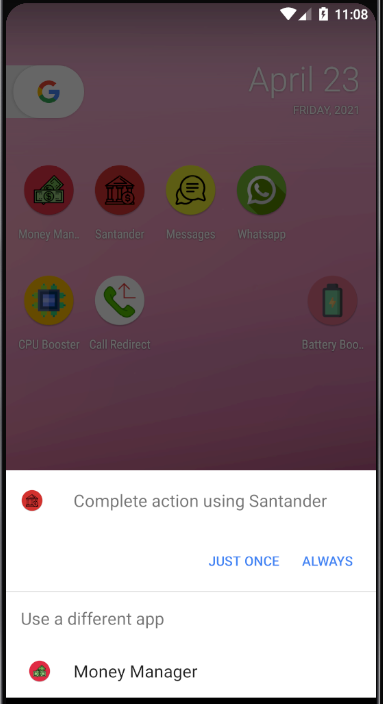
\includegraphics[width=0.35\textwidth]{graphics/activity_hijack.PNG}
        \caption{Choosing between activity of vulnerable app and malware.}
        \label{fig:activity_hijack}
    \end{wrapfigure}
        
    The vulnerable app for this challenge is Santander, a banking app. After they log in, the user can view details of fictitious bank accounts and can make fictional payments to another account, which will decrease the balance one of the accounts displayed in the app.
    
    Santander has an intent filter for its Login activity so that the user can click on special link that starts the bank app to make a payment. The link contains details of the recipient of the payment, such that these details are already filled in when the app launches and therefore making the payment easier. An implicit intent with this link can be sent from another app. It will match Santander's intent filter and start the Login activity to authenticate the user, before going to the payment screen.

    The attacker decompiled the Santander app to see the code for the Login activity and its intent filter. They made an activity in the Money Manager malware that looks identical to the one in Santander, and added to it an intent filter. Money Manager is an app for tracking and categorising one's income and expenses, but it does not have full functionality.
    
    When you open the app, the user sees a Loading screen, which sends an implicit intent to start the Login activity when it ends. There will be two filters that match with this intent, and therefore the user will be asked to pick between Santander and Money Manager, as you can see in figure \ref{fig:activity_hijack}. Both are financial apps, and Money Manager has a similar icon and colour theme, and therefore a careless user might select the malware. Money Manager's Login activity looks identical to Santander's, so the user types in their credentials, which the malware can then send to the attacker. To make it as if nothing suspicious happened, it will say the credentials are incorrect and then start the legitimate Login activity with an explicit intent.
    
    \subsubsection{Security Levels}
        \label{subsubsec:activity_hijack_security_levels}
        
    When sending intents to start an activity or service, you cannot protect them with a permission like you can when you send a broadcast and as we did in subsection \ref{subsubsec:broadcast_theft_security_levels}. Therefore, in the Impossible security level, the solution to fix the vulnerability is for the Santander Loading activity to use an explicit intent to start the Login activity. By doing this, the intent can not be sent to the malware. Explicit intents should be used for communication between components of the same app.

    However, when the user clicks on a link in another app to make a payment, the malware's intent filter will still match that implicit intent and the attack could succeed. For this case, the solution is to use App Links such that when a user clicks on a web link, they are either taken to a web page in a browser or they are taken to an activity in your app \cite{android_app_links}. These are not implemented in the Santander app at the current moment.
    
    \subsection{Content Provider URI Hijacking}
        \label{subsec:provider_uri_hijacking}
        
   In section \ref{sec:inter_component_communication} we saw that intents can transmit data using a URI. These URIs can point to data stored using a Content Provider. When declaring a Content Provider in the manifest file, the developer can set the \lstinline|android:grantUriPermissions| tag of the \lstinline|<provider>| element to true. This means that the content provider can allow temporary access to data linked to in a URI in an intent for a component in another app that received that intent. Therefore, external apps can access the content, even if the provider is not exported and thus not normally accessible by external apps.
    
    In order to do this, the intent that transmits the URI link must have the \lstinline|FLAG_GRANT_READ_URI_PERMISSION| or \lstinline|FLAG_GRANT_WRITE_URI_PERMISSION| flags added to it. If this intent is an implicit intent and is intercepted by a malicious component, then that component can read the data and perhaps modify it.
    
    \subsubsection{Implementation}
        \label{subsubsec:provider_uri_hijack_implementation}
        
    The vulnerable app for this challenge is Whatsapp, an internet messaging app named after the popular real world app. This app lets you view some hard-coded chats, it does not have real functionality. These chats are accessed by the app through its content provider, that is not exported, but that has \lstinline|android:grantUriPermissions| set to true in its manifest. The user can click on a button to go to another activity where they can select what chats they want to delete. When they click the delete button, the activity will send an implicit intent that contains the selection of chats, a URI to where chats are stored in the provider, and flags for temporary read and write permissions. This intent is received by a service of Whatsapp, which is responsible for accessing the provider and deleting the messages.
    
    Because this intent is implicit, it can be intercepted by the malware, which is the SMS Messages app in this case. This app only reads SMS messages on the device, it can not send new messages. The malware contains a service with an intent filter identical to that of the Whatsapp service. The malicious service will get the intent, and because the intent has temporary access flags, the malicious service can query the Whatsapp content provider and read messages. You can see these messages in the malware's log in figure \ref{fig:malware_log} on page \pageref{fig:malware_log}. Because Whatsapp's provider is not exported, if the malware queried the provider without having that intent, an exception would be thrown.
    
    \subsubsection{Security Levels}
        \label{subsubsec:provider_uri_hijack_security_levels}
        
    This challenge only has Low, High and Impossible security levels. In the High level, the provider is not exported and has not enabled temporary permissions overall. However, temporary permissions are enabled only for the path where chats are stored. Although the rest of the data in the provider can not be accessed by other apps, the data in this path can still be accessed by any component with a temporary permission. The temporary permission is still transmitted through the implicit intent sent by the Delete activity in Whatsapp.
    
    In the Impossible level, the intent sent by the Delete activity, which contains URIs to messages and has temporary permission flags, is sent as an explicit intents. The Messages malware can not get these intents and therefore can not get permission to access the provider. If it tries to query the provider, an exception will be thrown.
    
    \section{Testing}
        \label{sec:testing}
        
    The testing for the project was done using manual acceptance tests, which are documented in table \ref{table:tests}. These tests consist of using the apps of the project as the final user would and observing if the software behaves as expected. They check to see that the software fulfills the System Requirements. They were conducted on both a Pixel 3 emulator with Android 7.1 and a Huawei P10 Lite with Android 8.0. In table \ref{table:tests}, the tests with a number followed by a "*" are actually a set of tests, one for each challenge, but they are described as one to save space.
    
    We chose to do the tests manually instead of automating them due to time constraints and technical reasons. The project was being behind schedule, and writing automated systems tests would have taken time that was used to implement more features and challenges. Moreover, to test the communication between malware and vulnerable app, we would need to test if an intent sent by an app is received by a specific app. It is possible to test that an app sends certain intents \cite{testing_intents}, but we have not been able to find online any way to also test that a certain app receives the intent. Finally, the product is not complex enough to make manual testing impractical.
    
    \begin{center}
        \begin{longtable}{|p{0.4cm} |p{5.2cm} |p{7.4cm} |}
        \caption{Manual acceptance tests related to the DVM-ICC app in general.} \label{table:tests} \\
        
        \hline \multicolumn{1}{|c|}{\textbf{Test}} & \multicolumn{1}{c|}{\textbf{Steps}} & \multicolumn{1}{c|}{\textbf{Expected Outcome}} \\ \hline 
        \endfirsthead
        
        \multicolumn{3}{c}%
        {{\bfseries \tablename\ \thetable{} -- continued from previous page}} \\
        \hline \multicolumn{1}{|c|}{\textbf{Test}} & \multicolumn{1}{c|}{\textbf{Steps}} & \multicolumn{1}{c|}{\textbf{Expected Outcome}} \\ \hline 
        \endhead
        
        \hline \multicolumn{3}{|r|}{{Continued on next page}} \\ \hline
        \endfoot
        
        \hline \hline
        \endlastfoot
        
         \hline
         1 & Open the app. & On the first menu, you can scroll through the Introduction and Info pages. \\
         \hline
         2 & Open the app and click on the Challenges button. & The Challenges page has five buttons with the following texts: Broadcast Theft, Broadcast Theft - DOS, Broadcast Theft - MITM, Activity Intent Hijack and Content Provider URI Hijack. \\
         \hline
         3 & In any challenge, go to the Manifests page. & The Manifests page contains the correct Manifest and code snippets for every app in the project. \\
         \hline
         4 & In any challenge, click on the help icon. & No new activity opens and a warning appears. \\
         \hline
         5 & In any challenge, click on the Instructions button. & The Instructions page says that instructions are not available yet.\\
         \hline
         6 & In any challenge, click on the Questions button, answer the first two questions correctly then click on the Help button. & The Security Levels info activity starts, and it contains the correct explanation, full Manifest and relevant code snippets for all security levels of the selected challenge.\\
         \hline
         7 & In any challenge, click on the Questions button, answer the first two questions correctly then click on the Instructions button. & The Instructions page displays the correct instructions for completing that challenge.\\
         \hline
         8 & In any challenge, click on the Questions button, answer all but one question correctly then click on the Trophy button. & The Challenge Conclusion page opens, but tells you to complete the challenge to unlock the conclusion.\\
         \hline
         9 & In any challenge, click on the Questions button, answer all questions correctly then click on the Trophy button. & The Challenge Conclusion page opens and it shows an explanation and commentary for the chosen challenge.\\
         \hline
         10* & In all challenges, go to the Info page. & The Info page has the correct description for the attack and vulnerability of the selected challenge. \\
         \hline
         11* & In all challenges, click on the Questions button. & The Questions page contains two questions for identifying the vulnerable app and malware, respectively, a question for the flag of each security level, except the impossible level, of the selected challenge, and two questions for identifying the lines of code that introduce the vulnerability and attack, respectively. \\
         \hline
         12* & In all challenges, click on the Questions button. Type in wrong answers for all questions and click each submit button. & The submit buttons do not change. All question inputs are still enabled and their border turns red. \\
         \hline
         13* & In all challenges, click on the Questions button. Type in the correct answer for the selected challenge for all questions and click each submit button. & The submit buttons become outlined, their border and text is green, their text says "Completed" and they are not clickable anymore. The question inputs can not be re-edited and the correct answers can still be seen. \\
         \hline
         14* & In all challenges, for any security level, disable the malware and clear its log. Use the apps according the challenge's instructions. & The log of the malware is still empty, meaning that attack did not happen. \\
         \hline
         15* & In all challenges, for all security levels, enable the malware and clear its log. Use the apps according the challenge's instructions. & The log of the malware contains the correct flag for that security level, as well as any data stolen from the vulnerable app. There may be other expected outcomes in regards to how the malware or vulnerable app behaves, depending on the challenge and the security level.\\
         \hline

        \end{longtable}
    \end{center}
    